\chapter{Entrando en el mundo de \LaTeX}
\section*{$\odot$ Primeros Pasos}
Esta es una introducción a Latex. La unión entre el conjunto $A$ y $B$ se denota por $A\cup B$.
\begin{displaymath}
N(A\cup B)=N(A)+N(B)-N(A\cap B).
\end{displaymath}
Donde $N(A)$ es el número de elementos del conjunto $A$. 
%Notas de Overleaf
%Escritura de subindices y supraindices (filosofia)
\section{Subíndice y Supraíndices}
Diferentes formas de uso de índices y supraíndices:
\begin{enumerate}
\item La potenciación; $x$ elevado a la $y$: $x^y$. 
\item La sucesión $a$ de $n$: $\{a_n\}$. 
\item Expresión algebraica: $(a+b)^{nx+n^2+z^2}$.
\item Combinación sucesión y término algebraico: $(a_n^2+12)^{3+x}$.
\item Recurrencias: $a^{a^{a^a}}$.
\item Índices en las cuatro esquinas: $^{A}_{B}X_{C}^{D}$.
\item Índices con elementos poco convencinales: $\oplus^{\lhd}$
\end{enumerate}
\newpage
Fracciones y Número combinatorio. 
\pagenumbering{arabic}
\begin{itemize}
\item Estilo 1: $\frac{a}{b}.$
\item Estilo 2: $\displaystyle\frac{a}{b}.$
\item Estilo 3: $\dfrac{a}{b}.$
\item El factorial de $n$: $n!\equiv n\times(n-1)\times(n-2)\times\cdots \times 2\times 1$, Ejemplo: $3!=3\times 2\times 1=6$.
\item Numero combinatorio de $n$ y $m$: $\displaystyle\binom{n}{m}:=\dfrac{n!}{m!(n-m)!}$.
\item Ejemplo fracción: $\bigg(\dfrac{a}{b}+1\bigg)^2$
\item Ejemplo final: $$\displaystyle \binom{(n+m)^{x+y}}{\sqrt[n]{\dfrac{x}{y}}}$$.
\end{itemize}
\section{Aritmética}
\begin{Def}
Se dice que $a$ divide $b$ si existe un entero $x$ tal que $b=ax$ y se denota por $a|b$.
\end{Def}
\begin{Teo}
\label{Referencia_Division}
Si $a|b$ y $b|c$ entonces $a|c$.
\end{Teo}
\begin{proof}
Como $a|b$ y $b|c$ entonces existen $n$ y $m$ tales que:
$$b=na,$$ 
$$c=mb.$$
De los anterior $c=mb=m(na)=ka$ donde $k=nm$ y entonces $a|c$.
\end{proof}
Obsevación: Como se aprecia en el Teorema \ref{Referencia_Division}, se sabe que $2|24$ puesto que $2|4$ y $4|24$.\\
Considere el siguiente polinomio:
$$p(x)=x^2+2x-5.$$
Evalue el polinomio anterior en $x=-e+1$.
\begin{align*}
p(-e+1)=&(-e+1)^2+2(-e+1)-5\\
=&e^2-2e+1-2e+2-5\\
=&e^2-4e-2.
\end{align*}
\section{Variable Compleja}
Se sabe que en variable compleja, la siguiente ecuación se sostiene:
\begin{equation}
\label{EcuacionCompleja}
e^{i\pi}=-1
\end{equation}
\sangria La ecuación \eqref{EcuacionCompleja} es interesante puesto que contiene los símbolos matemáticos más importantes contenidos en una sola ecuación.\\[1cm]
Este es un salto de línea.
\section{Matrices}
Diferentes formas de escribir una matriz:
\begin{enumerate}
\item Matriz 1:
\begin{displaymath}
\begin{matrix}
0 & 1\\
0 & 0
\end{matrix}
\end{displaymath}
\item Matriz 2:
\begin{displaymath}
A=
\begin{pmatrix}
0 & 1\\
0 & 0
\end{pmatrix}
=
\begin{Bmatrix}
0 & 1\\
0 & 0
\end{Bmatrix}
\end{displaymath}
\item Matriz 3:
\begin{displaymath}
\begin{bmatrix}
0 & 1\\
0 & 0
\end{bmatrix}
\end{displaymath}
\item Matriz 4:
\begin{displaymath}
\left (
\begin{matrix}
0 & 1\\
0 & 0
\end{matrix}
\right |
\end{displaymath}
\item Ejemplo:	 Demuestre que si
\begin{displaymath}
\begin{vmatrix}
a_{11} & a_{12} & \cdots & a_{1n}\\
a_{21} & a_{22} & \cdots & a_{2n}\\
\vdots & \vdots & \ddots &\vdots \\
a_{n1} & a_{n2} & \cdots & a_{nn}
\end{vmatrix}\neq -1
\end{displaymath}
\end{enumerate}
\newpage
\chapter{Imagenes en \LaTeX}
\section{Insertar Imágenes}
\sangria La siguiente imagen fue tomada de internet:\\
\begin{figure}[H]
\begin{center}
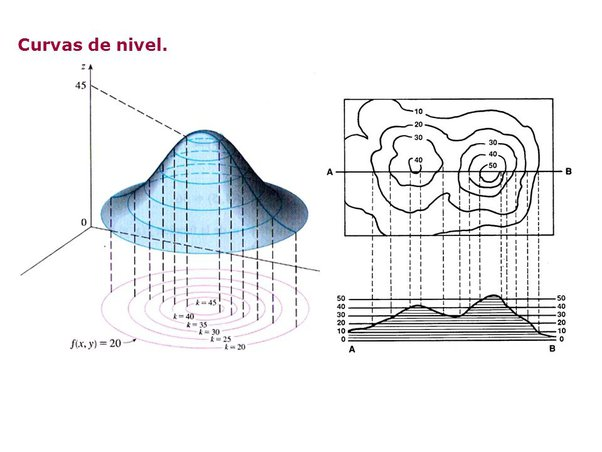
\includegraphics[scale=0.4]{Imagenes/Imagen1}
\caption{La imagen fue tomada de la pagina www.pagina.com}
\end{center}
\end{figure}
\lipsum[1-15]
\begin{figure}[H]
\begin{center}
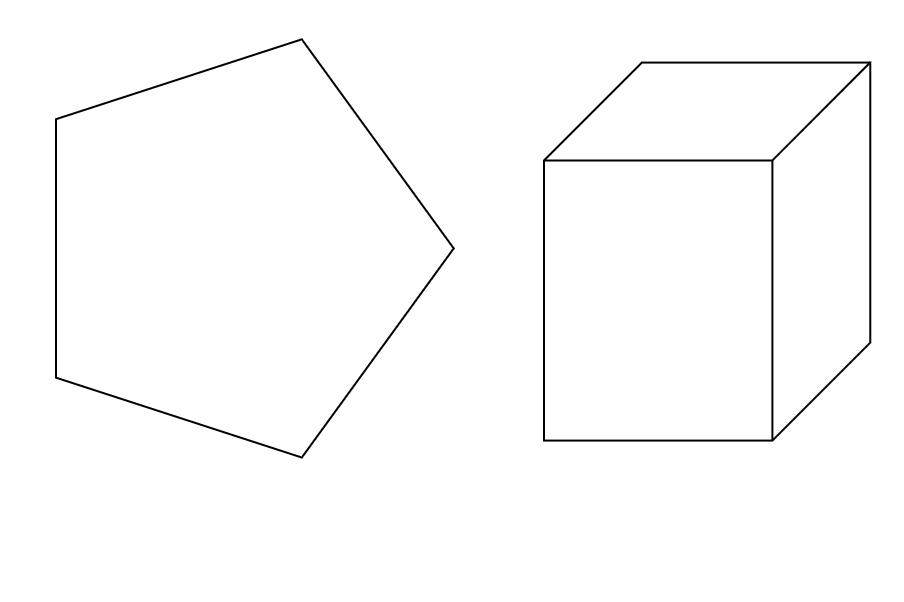
\includegraphics[scale=0.4]{Imagenes/Imagen2}
\caption{Imagen generada en Mathcha.}
\end{center}
\end{figure}
\tikzset{every picture/.style={line width=0.75pt}} %set default line width to 0.75pt        

\begin{tikzpicture}[x=0.75pt,y=0.75pt,yscale=-1,xscale=1]
%uncomment if require: \path (0,300); %set diagram left start at 0, and has height of 300

%Shape: Regular Polygon [id:dp6163162722543882] 
\draw   (226.86,124.21) -- (150.9,228.76) -- (27.99,188.83) -- (27.99,59.6) -- (150.9,19.67) -- cycle ;
%Shape: Cube [id:dp12455656353557121] 
\draw   (272,80.23) -- (320.94,31.29) -- (435.14,31.29) -- (435.14,171.34) -- (386.2,220.29) -- (272,220.29) -- cycle ; \draw   (435.14,31.29) -- (386.2,80.23) -- (272,80.23) ; \draw   (386.2,80.23) -- (386.2,220.29) ;

\end{tikzpicture}